%% Applied Energy (Elsevier) submission -- built on the elsarticle-num template.
%% Compile: pdflatex -> bibtex -> pdflatex -> pdflatex   (or: latexmk -pdf)
%% Figures: ../result (study output) and ./img (test-rig photo).
\documentclass[preprint,12pt]{elsarticle}

%% Use the option review to obtain double line spacing for markup:
%% \documentclass[preprint,review,12pt]{elsarticle}

\usepackage{amssymb}
\usepackage{amsmath}
\usepackage{booktabs}
\usepackage{siunitx}
\usepackage{lineno}
\usepackage[hidelinks]{hyperref}

%% graphicx is already loaded by elsarticle.cls; just point it at the figures.
\graphicspath{{../result/}{./img/}}
\DeclareMathOperator*{\argmax}{arg\,max}

\journal{Applied Energy}

\begin{document}

\begin{frontmatter}

\title{Data-Driven Sequential Decision-Making for Small Hydro Propeller Turbine
Performance Testing: Bayesian Optimization and Active Learning for Experiment
Reduction}

\author[a]{Siwakorn Suprasertchai}
\author[b]{Kornpaphop Ruttanawijit}
\author[a]{Yodchai Tiaple\corref{cor1}}
\ead{yodchai.ti@ku.th}
\cortext[cor1]{Corresponding author.}

\affiliation[a]{organization={Department of Maritime Engineering, Faculty of
International Maritime Studies, Kasetsart University, Sriracha Campus},
            city={Chonburi},
            country={Thailand}}
\affiliation[b]{organization={Department of Energy Technology, Faculty of
Engineering and Industry Technology, Rambhai Barni Rajabhat University},
            country={Thailand}}

\begin{abstract}
Constructing the efficiency map (hill chart) of a hydraulic turbine and locating
its best efficiency point (BEP) requires many physical experiments, each costly in
both time and labor. Existing approaches either couple surrogate models to
CFD-based geometric design or fit models to pre-collected test data under a fixed
sampling plan; the use of an adaptive policy to decide which physical experiments
to run, benchmarked against classical design of experiments on real measurements,
remains unaddressed. This work frames performance testing as a sequential decision
problem and compares six sampling policies: Bayesian optimization with an
upper-confidence-bound acquisition (BO-UCB), two Gaussian-process active-learning
policies (ALM and ALC), and random, grid, and Latin hypercube sampling. Sweeping
the experimental budget from 6 to 30 points over 20 random seeds, we evaluate every
policy against a 72-point baseline measured on a \SI{137}{\kilo\watt} small-hydro
propeller turbine. For reconstructing the full hill chart the active learners
dominate: ALC reaches $R^2 = 0.996$ and $\mathrm{MAPE} = 0.35\%$ from only 12
experiments (an 83.3\% reduction), whereas BO-UCB is the weakest at reconstruction
($R^2 = 0.921$). For locating the BEP the ranking inverts: BO-UCB identifies the
exact BEP node ($Q = \SI{0.8185}{\cubic\metre\per\second}$, $H = \SI{16.00}{\metre}$,
$\eta^\ast = 0.6973$) on every seed from 14 experiments (an 81\% reduction), while
all other policies plateau near $\Delta\eta \approx 10^{-2}$. Every separation is
confirmed by paired Wilcoxon signed-rank tests. These results show that the
acquisition function must match the deliverable: global fit is the wrong success
metric for BEP-directed testing, and BEP-directed sampling is the wrong tool for
building the map.
\end{abstract}

\begin{graphicalabstract}
\centering
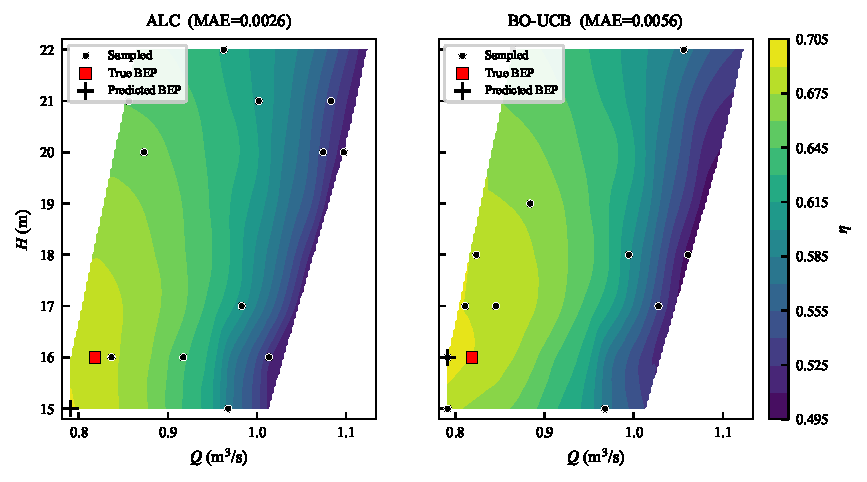
\includegraphics[width=0.9\linewidth]{fig_goal_contrast.pdf}
\end{graphicalabstract}

\begin{highlights}
\item Turbine performance testing is framed as a budget-constrained sequential decision problem.
\item Six sampling policies are benchmarked on 72 real propeller-turbine measurements.
\item Active learning reconstructs the full hill chart to $R^2\approx0.996$ using only 12 of the 72 test points.
\item Bayesian optimization locates the exact best efficiency point from only 14 test points.
\item The two objectives select opposite winners; the sampler must match the deliverable.
\end{highlights}

\begin{keyword}
Bayesian optimization \sep sequential experimental design \sep small hydropower
\sep propeller turbine \sep surrogate modeling \sep active learning
\end{keyword}

\end{frontmatter}

\linenumbers

%======================================================================
\section{Introduction}\label{sec:intro}
%======================================================================

\subsection{Background and motivation}
Small hydropower remains one of the most mature and dispatchable sources of
renewable electricity, and propeller-type reaction turbines are widely deployed in
run-of-river and low-head installations where the available head is modest but the
flow is comparatively large. The operational value of such a machine is governed by
its efficiency characteristic over the full envelope of discharge and head at which
it is expected to run. This characteristic is summarized by the efficiency map, or
hill chart, which expresses turbine efficiency as a function of the principal
operating variables and locates the best efficiency point (BEP)---the operating
condition at which the machine converts the available hydraulic power into shaft
power most effectively. Accurate knowledge of the hill chart and of the BEP
underpins site matching, control-system tuning, performance guarantees, and
condition monitoring throughout the service life of the unit.

Constructing a reliable hill chart from physical measurements is expensive. Each
test point requires the rig to be brought to a stable operating condition, the
instrumentation to settle, and repeated readings to be averaged, all under
controlled procedures. A densely sampled map of the kind used as ground truth in the
present study---comprising several dozen individual operating points across the
discharge--head plane---represents a substantial commitment of test-rig time,
energy, and labor. In commercial and research settings alike, this cost places a
practical ceiling on how finely the operating envelope can be characterized, and it
motivates a question that is fundamentally one of resource allocation: given a
limited budget of physical experiments, which operating points should be measured so
that the quantities of engineering interest are recovered as accurately as possible?
Propeller and other reaction turbines are the dominant choice in the low- and
ultra-low-head range, where compact run-of-river installations are increasingly
important for distributed renewable generation~\cite{zhou2017ultralowhead}, and
small-hydro units of this class have been deployed and characterized in
run-of-river settings in Thailand~\cite{phitaksurachai2017performance}. Standardized
model- and prototype-acceptance testing of such machines follows international
codes~\cite{iec60193}, whose controlled procedures are precisely what make each
measured operating point costly.

\subsection{The decision problem in turbine performance testing}
The question above is best framed not as a curve-fitting problem but as a sequential
decision-making problem under expensive evaluation. At each stage of a test
campaign, the engineer has already observed efficiency at a set of operating points
and must decide where to run the next experiment. The decision is made under
uncertainty, because the efficiency at untested conditions is unknown, and it is
made under a budget constraint, because every additional experiment consumes scarce
resources. A good decision policy allocates the limited budget to the points that
are most informative for the goal at hand, rather than spreading effort uniformly
across a region of the operating envelope that may be of little practical interest.
This framing matters because the goal of a test campaign is frequently not to
reconstruct the entire efficiency surface with uniform fidelity, but to determine
the operationally decisive quantities---above all the location and value of the BEP
and the shape of the high-efficiency region around it. A test plan optimized for
uniform global accuracy and a test plan optimized for locating the BEP are not the
same plan, and confusing the two can lead an otherwise careful study to measure the
wrong points. Recognizing turbine performance testing as a targeted,
budget-constrained decision process, rather than a passive data-collection exercise,
is the conceptual starting point of this work.

\subsection{Research gap}
Data-driven and surrogate-based methods for reducing the number of evaluations in
turbine engineering are now well established, but the existing literature addresses a
different problem from the one posed here. The dominant body of work couples
surrogate models---Gaussian process regression, polynomial response surfaces, or
neural networks---to computational fluid dynamics (CFD) and uses them to accelerate
the geometric design of runners and blades, validating the surrogate against further
CFD rather than against physical measurements~\cite{masood2021ml}. These studies
typically operate over a small number of geometric design variables and treat the
expensive evaluation as a simulation, not a laboratory test. A second, more recent
strand applies machine learning to experimental turbine data to predict efficiency,
but it fits models to data that have already been collected and does not use the
model to decide which experiments to run; the sampling plan is fixed in
advance~\cite{besni2025ml}. Classical design of experiments in turbine work---central
composite designs, factorial designs, Latin hypercube designs---is likewise
specified before any testing begins and is non-adaptive~\cite{betancour2023vortex}.
What is absent is a study that treats the construction of a turbine performance map
from real physical experiments as an adaptive, budget-constrained decision process,
and that benchmarks an adaptive policy against the classical fixed designs on the
specific task of locating the BEP. The present work addresses this gap directly. It
uses a measured ground-truth dataset for a small-hydro propeller turbine, frames
test-point selection as sequential decision-making, and compares adaptive
Gaussian-process policies---Bayesian optimization and two active-learning
designs---against random, grid, and Latin hypercube sampling across a sweep of
experimental budgets, with both the full hill chart and the BEP as explicit decision
targets.

\subsection{Contributions and organization}
The contributions of this paper are as follows.
\begin{enumerate}
\item We formulate the construction of a small-hydro propeller-turbine performance
map as a sequential, budget-constrained decision problem with two distinct
objectives---uniform surface reconstruction and best-efficiency-point
identification---and we make explicit why these objectives demand different sampling
strategies and different success metrics.
\item We benchmark six sampling policies---a Bayesian optimization (BO-UCB) policy,
two Gaussian-process active-learning policies (ALM and ALC), and three classical
design-of-experiments baselines (random, grid, and Latin hypercube sampling)---on a
measured ground-truth dataset of 72 physical experiments, sweeping the budget from 6
to 30 experiments and evaluating every policy across 20 random seeds so that the
comparison reflects expected behavior rather than a single fortunate run.
\item We show that the two objectives select opposite winners. The active learners
reconstruct the full hill chart to $R^2 \geq 0.99$ from as few as 10 experiments and
to $R^2 \approx 0.996$ at 12 (an 83.3\% reduction), while the Bayesian policy is the
weakest map-builder; conversely, the Bayesian policy locates the exact BEP node on
every seed from 14 experiments (an 81\% reduction), while every other policy plateaus
near $\Delta\eta \approx 10^{-2}$. We confirm each separation with paired Wilcoxon
signed-rank tests and argue that global accuracy is the wrong success criterion for a
BEP-directed campaign.
\item We quantify the achievable experiment reduction through a budget sweep from 6
to 30 experiments, identify the very-low-budget regime ($n < 8$) in which
model-based policies degrade and space-filling designs are the safer choice, and
derive tiered practical guidance that matches the sampling policy to the deliverable.
\end{enumerate}
The remainder of the paper is organized as follows. Section~\ref{sec:related}
reviews surrogate and machine-learning models for turbine performance, classical
design of experiments, and Bayesian optimization as a framework for adaptive
experimental design, and positions the present work against the closest prior art.
Section~\ref{sec:problem} formulates the performance-mapping task as a sequential
decision problem and defines the decision objective. Section~\ref{sec:method}
describes the experimental dataset, the Gaussian-process surrogate and the adaptive
sampling policies, the initialization, the baseline designs, and the evaluation
protocol. Section~\ref{sec:results} reports the results. Section~\ref{sec:discussion}
discusses the findings, their decision-support implications, and the limitations of
the study, and concludes.

%======================================================================
\section{Related Work}\label{sec:related}
%======================================================================

\subsection{Surrogate and machine-learning models for turbine performance maps}
Surrogate modeling has become a standard tool for reducing the computational cost of
turbine analysis and design. The representative contribution in the hydropower
context is the machine-learning surrogate of Masood et al.~\cite{masood2021ml}, who
coupled a Gaussian process model to CFD to accelerate the simulation-driven
optimization of a Kaplan turbine runner. Their surrogate is trained on CFD
evaluations over a parametric geometric design space and is validated against
further CFD; the reported outcome is a substantial improvement in the efficiency of
the optimized design relative to the baseline geometry, achieved at a fraction of the
computational cost of exhaustive simulation. This work is emblematic of a large
family of studies in which the expensive evaluation is a numerical simulation, the
design variables describe machine geometry, and the validation reference is itself
computational. The objective in these studies is design improvement, not the
empirical characterization of an existing machine from laboratory measurements. A
more recent line of work brings machine learning to bear on experimental turbine
data. Besni et al.~\cite{besni2025ml} developed machine-learning models to predict
the efficiency of Francis-type hydraulic turbines using data obtained from
comprehensive model-acceptance performance testing, combining experimental and
numerical information in the predictive model. This is closer in spirit to the
present study because the data are physical measurements rather than simulations. The
decisive difference is that the predictive model is fitted to a sampling plan that
has been fixed in advance; the model does not participate in deciding which operating
points to test, and the number of experiments is not itself the object of
optimization. The same observation applies to the broader literature on
efficiency-map and hill-chart fitting, in which measured points are interpolated or
regressed after the fact to yield a continuous characteristic. Beyond these
representative cases, a rapidly growing body of work applies machine learning to the
performance characterization of hydraulic machines. Data-driven models have been used
to predict the best-efficiency operating point and the complete performance curves of
pumps operating as turbines~\cite{telikani2023pat,yu2024pat}, and to estimate turbine
power output directly from operating data~\cite{malakouti2023turbinepower}. The
broader role of artificial intelligence in turbomachinery design, validation, and
condition monitoring---including Gaussian-process surrogates and Bayesian
optimization---has recently been surveyed~\cite{zou2024aiturbomachinery}, and hybrid
schemes that combine neural networks with physics-based off-design analysis
illustrate the same trend in adjacent turbomachinery~\cite{talebi2022microgt}. In
every case the surrogate is fitted to a predetermined dataset; it does not decide
which experiments to perform.

\subsection{Classical design of experiments in turbine experimentation}
Design of experiments (DOE) provides the classical toolkit for choosing where to
sample an input space when each observation is costly. In turbine and pump research
the dominant approach is response surface methodology~\cite{box1951rsm} built on
central composite designs, which place experimental points at factorial corners,
axial points, and a center point to support the fitting of a second-order polynomial
model. Betancour et al.~\cite{betancour2023vortex}, for example, used a central
composite design to optimize the runner of a gravitational vortex turbine, monitoring
the response through CFD and validating the optimum experimentally; comparable
central composite designs appear throughout the pump-as-turbine and mixed-flow
literature. Latin hypercube sampling, introduced by McKay et al.~\cite{mckay1979lhs},
is the other widely used design, valued for its space-filling properties and its even
projection of points onto each input dimension. Full or fractional factorial grids
and uniform random sampling complete the set of conventional choices. The defining
feature of all of these designs is that they are non-adaptive: the complete set of
sampling locations is determined before any measurement is taken, using only prior
knowledge of the input ranges and no information from the responses themselves. This
is appropriate when the goal is to characterize the whole input space uniformly or to
fit a low-order global model, and it is the reason space-filling designs perform
strongly on global reconstruction metrics. It is less appropriate when the goal is
concentrated on a particular feature of the response, such as the location of an
optimum, because the budget is spent uniformly rather than where the feature lies.
Recent applications confirm the continued prevalence of these designs in energy and
turbomachinery engineering: central composite designs coupled to computational fluid
dynamics have been used to optimize turbine-duct geometry~\cite{taghinezhad2023duct}.
To soften the strictly non-adaptive nature of classical space-filling designs,
adaptive Latin hypercube schemes have been proposed that add samples sequentially in
regions of high surrogate deviation~\cite{borisut2023adaptivelhs}; such schemes move
partway toward the adaptive policy studied here while remaining variance-driven
rather than objective-driven.

\subsection{Bayesian optimization and adaptive experimental design}
Bayesian optimization (BO) is a framework for the sequential, model-based
optimization of expensive black-box functions~\cite{jones1998ego,shahriari2016boreview}.
It maintains a probabilistic surrogate of the unknown function---most commonly a
Gaussian process~\cite{rasmussen2006gpml}---and uses an acquisition function derived
from the surrogate's posterior to decide where to evaluate next, balancing
exploitation of regions believed to be near-optimal against exploration of regions
where the surrogate is uncertain. The Expected Improvement criterion of Jones et
al.~\cite{jones1998ego} and the upper-confidence-bound family~\cite{srinivas2012ucb}
are the canonical acquisition functions, and the approach has been applied across
machine-learning hyperparameter tuning~\cite{snoek2012practicalbo} and a wide range
of engineering design tasks. Of particular relevance here is the use of BO not for
optimization per se but as a policy for adaptive experimental design. Greenhill et
al.~\cite{greenhill2020boreview} review this perspective explicitly, framing BO as an
automated decision policy for choosing experiments and contrasting it with classical
fixed designs; benchmark studies in experimental materials
science~\cite{liang2021benchmarkbo} likewise compare BO against space-filling and
random designs across diverse real datasets. The consistent finding across this
literature is that adaptive policies excel when the objective is to find an optimum
efficiently, precisely because they deliberately concentrate sampling near the
optimum and decline to spend budget on uninformative regions---at the expense of
global model accuracy. This exploitation behavior is central to interpreting the
results of the present study. Within fluid machinery specifically, Bayesian
optimization and Gaussian-process surrogates have been applied to one-dimensional
turbomachinery design through transfer learning~\cite{chen2022transferbo}, to
multi-objective aerodynamic shape optimization of airfoils~\cite{liu2022airfoilbo}, to
coupled aerodynamic and aeroacoustic blade design~\cite{lim2022aeroacoustic}, and to
high-dimensional aero-structural compressor-blade design~\cite{pretsch2025compressor}.
More generally, active-learning strategies that construct surrogate models with the
fewest possible expensive evaluations~\cite{guo2024activelearning} share the
objective-directed sampling philosophy adopted here. These applications are
predominantly simulation-based and geometry-oriented; their adaptation to the
selection of physical operating points on a measured turbine, with the BEP as the
explicit target, is the contribution of the present work.

\subsection{Positioning of the present work}
Table~\ref{tab:positioning} positions the present study against the closest prior art
along four axes: the nature of the data, the method, the optimization target, and
whether the approach is benchmarked against classical designs. The combination
addressed here---physical experimental data, adaptive Gaussian-process policies
(Bayesian optimization and active learning) benchmarked against random, grid, and
Latin hypercube designs, on a small-hydro propeller turbine, with the BEP as the
explicit target---does not appear in the existing literature. The present work does
not claim to be the first application of Bayesian optimization to a turbine; it claims
novelty in this specific combination and, more importantly, in the decision-level
finding that the sampling policy must be matched to the deliverable:
exploitation-driven sampling wins for BEP identification despite inferior global
metrics, while uncertainty-driven active learning wins for hill-chart reconstruction.

\begin{table}[t]
\centering
\caption{Positioning relative to the closest prior work.}
\label{tab:positioning}
\small
\begin{tabular}{@{}p{2.4cm}p{2.3cm}p{2.6cm}p{2.4cm}p{2.0cm}@{}}
\toprule
Study & Data source & Method & Target & Benchmarked vs.\ classical DOE \\
\midrule
Masood et al.\ (2021) & CFD & GP surrogate + optimization & Runner geometry design & No \\
Besni et al.\ (2025) & Experiment (model test) & ML efficiency prediction & Efficiency prediction & No \\
Betancour et al.\ (2023) & CFD + experiment & RSM / CCD & Runner geometry design & Single design family \\
Greenhill et al.\ (2020) & Various (review) & BO / adaptive design & Generic optimization & Conceptual \\
\textbf{This work} & \textbf{Experiment (test rig)} & \textbf{Adaptive GP policies (BO, ALM, ALC)} & \textbf{BEP localization + map} & \textbf{Random, Grid, LHS} \\
\bottomrule
\end{tabular}
\end{table}

%======================================================================
\section{Problem Formulation}\label{sec:problem}
%======================================================================

\subsection{Performance map and best efficiency point}
Let the operating condition of the turbine be described by the discharge $Q$ and the
head $H$, and let $\eta(Q, H)$ denote the measured efficiency at that condition. The
performance map is the function $\eta$ defined over the feasible operating domain
$\mathcal{X}$, a subset of the $(Q, H)$ plane, which in the present study spans
$Q \in [0.791, 1.123]\ \si{\cubic\metre\per\second}$ and
$H \in [15, 22]\ \si{\metre}$. The best efficiency point is the maximizer of
efficiency over this domain:
\begin{equation}
(Q^\ast, H^\ast) = \argmax_{(Q,H)\in\mathcal{X}} \eta(Q,H), \qquad
\eta^\ast = \eta(Q^\ast, H^\ast).
\label{eq:bep}
\end{equation}
In the measured ground-truth dataset the BEP is located at
$Q = \SI{0.8185}{\cubic\metre\per\second}$, $H = \SI{16.00}{\metre}$ (guide-vane
angle \ang{37.5}), with $\eta^\ast = 0.6973$, in the low-discharge, low-head corner
of the envelope where the efficiency ridge is highest. The efficiency surface is
smooth and unimodal in the high-efficiency region, with a single broad ridge
descending toward a low-efficiency corner at high discharge (efficiency falling to
0.497); this structure is typical of low-head propeller machines.
Fig.~\ref{fig:gt3d} presents the measured efficiency surface of this turbine in three
dimensions, and Fig.~\ref{fig:gt2d} shows the same data as a contour map of the
discharge--head plane with the BEP marked.

\begin{figure}[t]
\centering
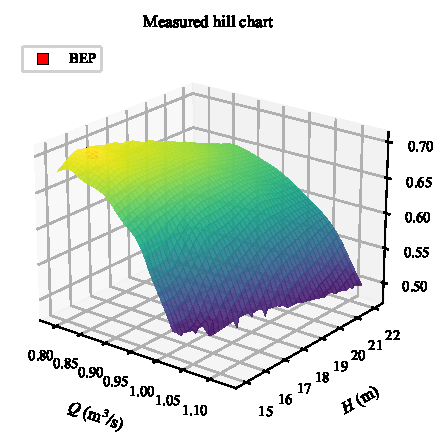
\includegraphics[width=0.66\linewidth]{fig_ground_truth_3d.pdf}
\caption{Measured ground-truth efficiency surface of the \SI{137}{\kilo\watt}
propeller turbine (72 experimental points) in the discharge--head plane.}
\label{fig:gt3d}
\end{figure}

\begin{figure}[t]
\centering
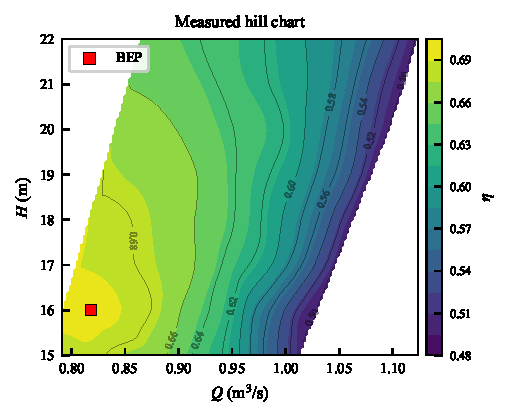
\includegraphics[width=0.64\linewidth]{fig_ground_truth_2d.pdf}
\caption{Measured ground-truth efficiency contour map with the experimental points
and the best efficiency point (BEP).}
\label{fig:gt2d}
\end{figure}

The true function $\eta$ is observable only through physical experiments. Each
experiment at a chosen condition $(Q_i, H_i)$ returns a measurement
$y_i = \eta(Q_i, H_i) + e_i$, where $e_i$ captures measurement and repeatability
error. Experiments are expensive, so the number that can be performed is limited to a
budget $N$ that is small relative to the resolution at which the map would ideally be
known.

\subsection{Sequential decision formulation}
We cast the construction of the performance map as a sequential decision problem.
After $t$ experiments the state is the set of observed condition--efficiency pairs
$\mathcal{D}_t = \{(Q_i, H_i, y_i)\}_{i=1}^{t}$. An action is the choice of the next
operating condition $(Q_{t+1}, H_{t+1}) \in \mathcal{X}$ at which to run an
experiment; each operating point is specified by $(Q, H)$, which fixes the
corresponding guide-vane setting on the test manifold. A policy $\pi$ is a rule that
maps the current state to the next action, $(Q_{t+1}, H_{t+1}) = \pi(\mathcal{D}_t)$.
The process begins from an initial design of $n_0$ points and proceeds until the
budget $N$ is exhausted. This formulation unifies the methods compared in this paper.
The classical designs correspond to non-adaptive policies whose actions do not depend
on the observed efficiencies: random sampling draws each condition independently from
$\mathcal{X}$, grid sampling places conditions on a fixed lattice, and Latin hypercube
sampling selects a space-filling set with even one-dimensional projections. Bayesian
optimization corresponds to an adaptive policy: it maintains a surrogate model of
$\eta$ given $\mathcal{D}_t$ and chooses each action by maximizing an acquisition
function that depends on the surrogate's posterior mean and variance, so that the next
experiment is selected in light of everything observed so far. The distinction between
non-adaptive and adaptive policies is the central methodological variable of the
study.

\subsection{Decision objective and the inadequacy of global fit}
The choice of objective determines which policy is good. Two objectives must be
distinguished. The first is global reconstruction: to recover the entire surface
$\eta$ over $\mathcal{X}$ with uniform accuracy, measured by aggregate error
statistics such as the mean absolute error or the coefficient of determination
computed over the whole domain. The second is BEP identification: to determine
$(Q^\ast, H^\ast)$ and $\eta^\ast$, and to characterize the high-efficiency region
around the optimum, as accurately as possible within the budget. These objectives are
not aligned. A policy optimized for global reconstruction spreads its budget evenly
and is rewarded for accuracy in regions of the operating envelope---such as the
low-efficiency, high-discharge corner---that are of little operational interest. A
policy optimized for BEP identification concentrates its budget near the optimum and
is content to model the uninteresting regions poorly. Consequently, the global error
of a BEP-directed policy can be large even when its localization of the optimum is
exact, and conversely a space-filling design can achieve excellent global error while
placing no experiments close enough to the true optimum to resolve it precisely. The
results of Section~\ref{sec:results} demonstrate exactly this reversal. It follows
that global reconstruction metrics are the wrong success criterion for a BEP-directed
campaign. We therefore evaluate every policy under both objectives---global
reconstruction metrics for the hill chart and localization error for the BEP---and
rank each policy only under the objective it is designed to serve. The formal
definitions of these metrics are given in Section~\ref{sec:eval}.

%======================================================================
\section{Methodology}\label{sec:method}
%======================================================================

\subsection{Experimental dataset and test rig}
The ground-truth dataset consists of 72 measured operating points for a small-hydro
propeller turbine, organized as eight constant-head test series at heads of 15, 16,
17, 18, 19, 20, 21, and \SI{22}{\metre}, each comprising a sweep of guide-vane
openings and the corresponding discharge. The measured variables at each point are the
guide-vane angle, the discharge, the generator power, the mechanical power, and the
resulting overall efficiency. Discharge spans 0.791 to
\SI{1.123}{\cubic\metre\per\second} and overall efficiency spans 0.497 to 0.6973
across the envelope. These 72 points constitute the reference against which all
sampling policies are evaluated and are treated throughout as ground truth.

The turbine under study is an axial-flow propeller (bulb) turbine developed for
low-head small-hydro applications in Thailand under the Electricity Generating
Authority of Thailand (EGAT) Small Hydro Power Research and Development Project, the
same machine family later summarized by Phitaksurachai et
al.~\cite{phitaksurachai2017performance}. The specific unit analyzed here is the
\SI{137}{\kilo\watt}-rated turbine designed for the 15--\SI{20}{\metre} head class.
The runner has four fixed blades of \SI{0.4}{\metre} diameter with a hub-to-tip ratio
of 0.35, fixed to the hub at \ang{40} in the radial plane; the blade geometry is a
marine-propeller form with a reversed mean camber line derived from a NACA 4410
airfoil section. Flow is regulated by twelve adjustable guide vanes, and the machine
is a reaction turbine fitted with a draft tube. The turbine shaft is directly coupled,
within the bulb, to a \SI{160}{\kilo\watt} induction generator running at
\SI{1000}{rpm}. The sub-megawatt rating and low-head design place the unit firmly in
the small-hydro class. Fig.~\ref{fig:rig} shows the unit installed on the performance
test rig.

\begin{figure}[t]
\centering
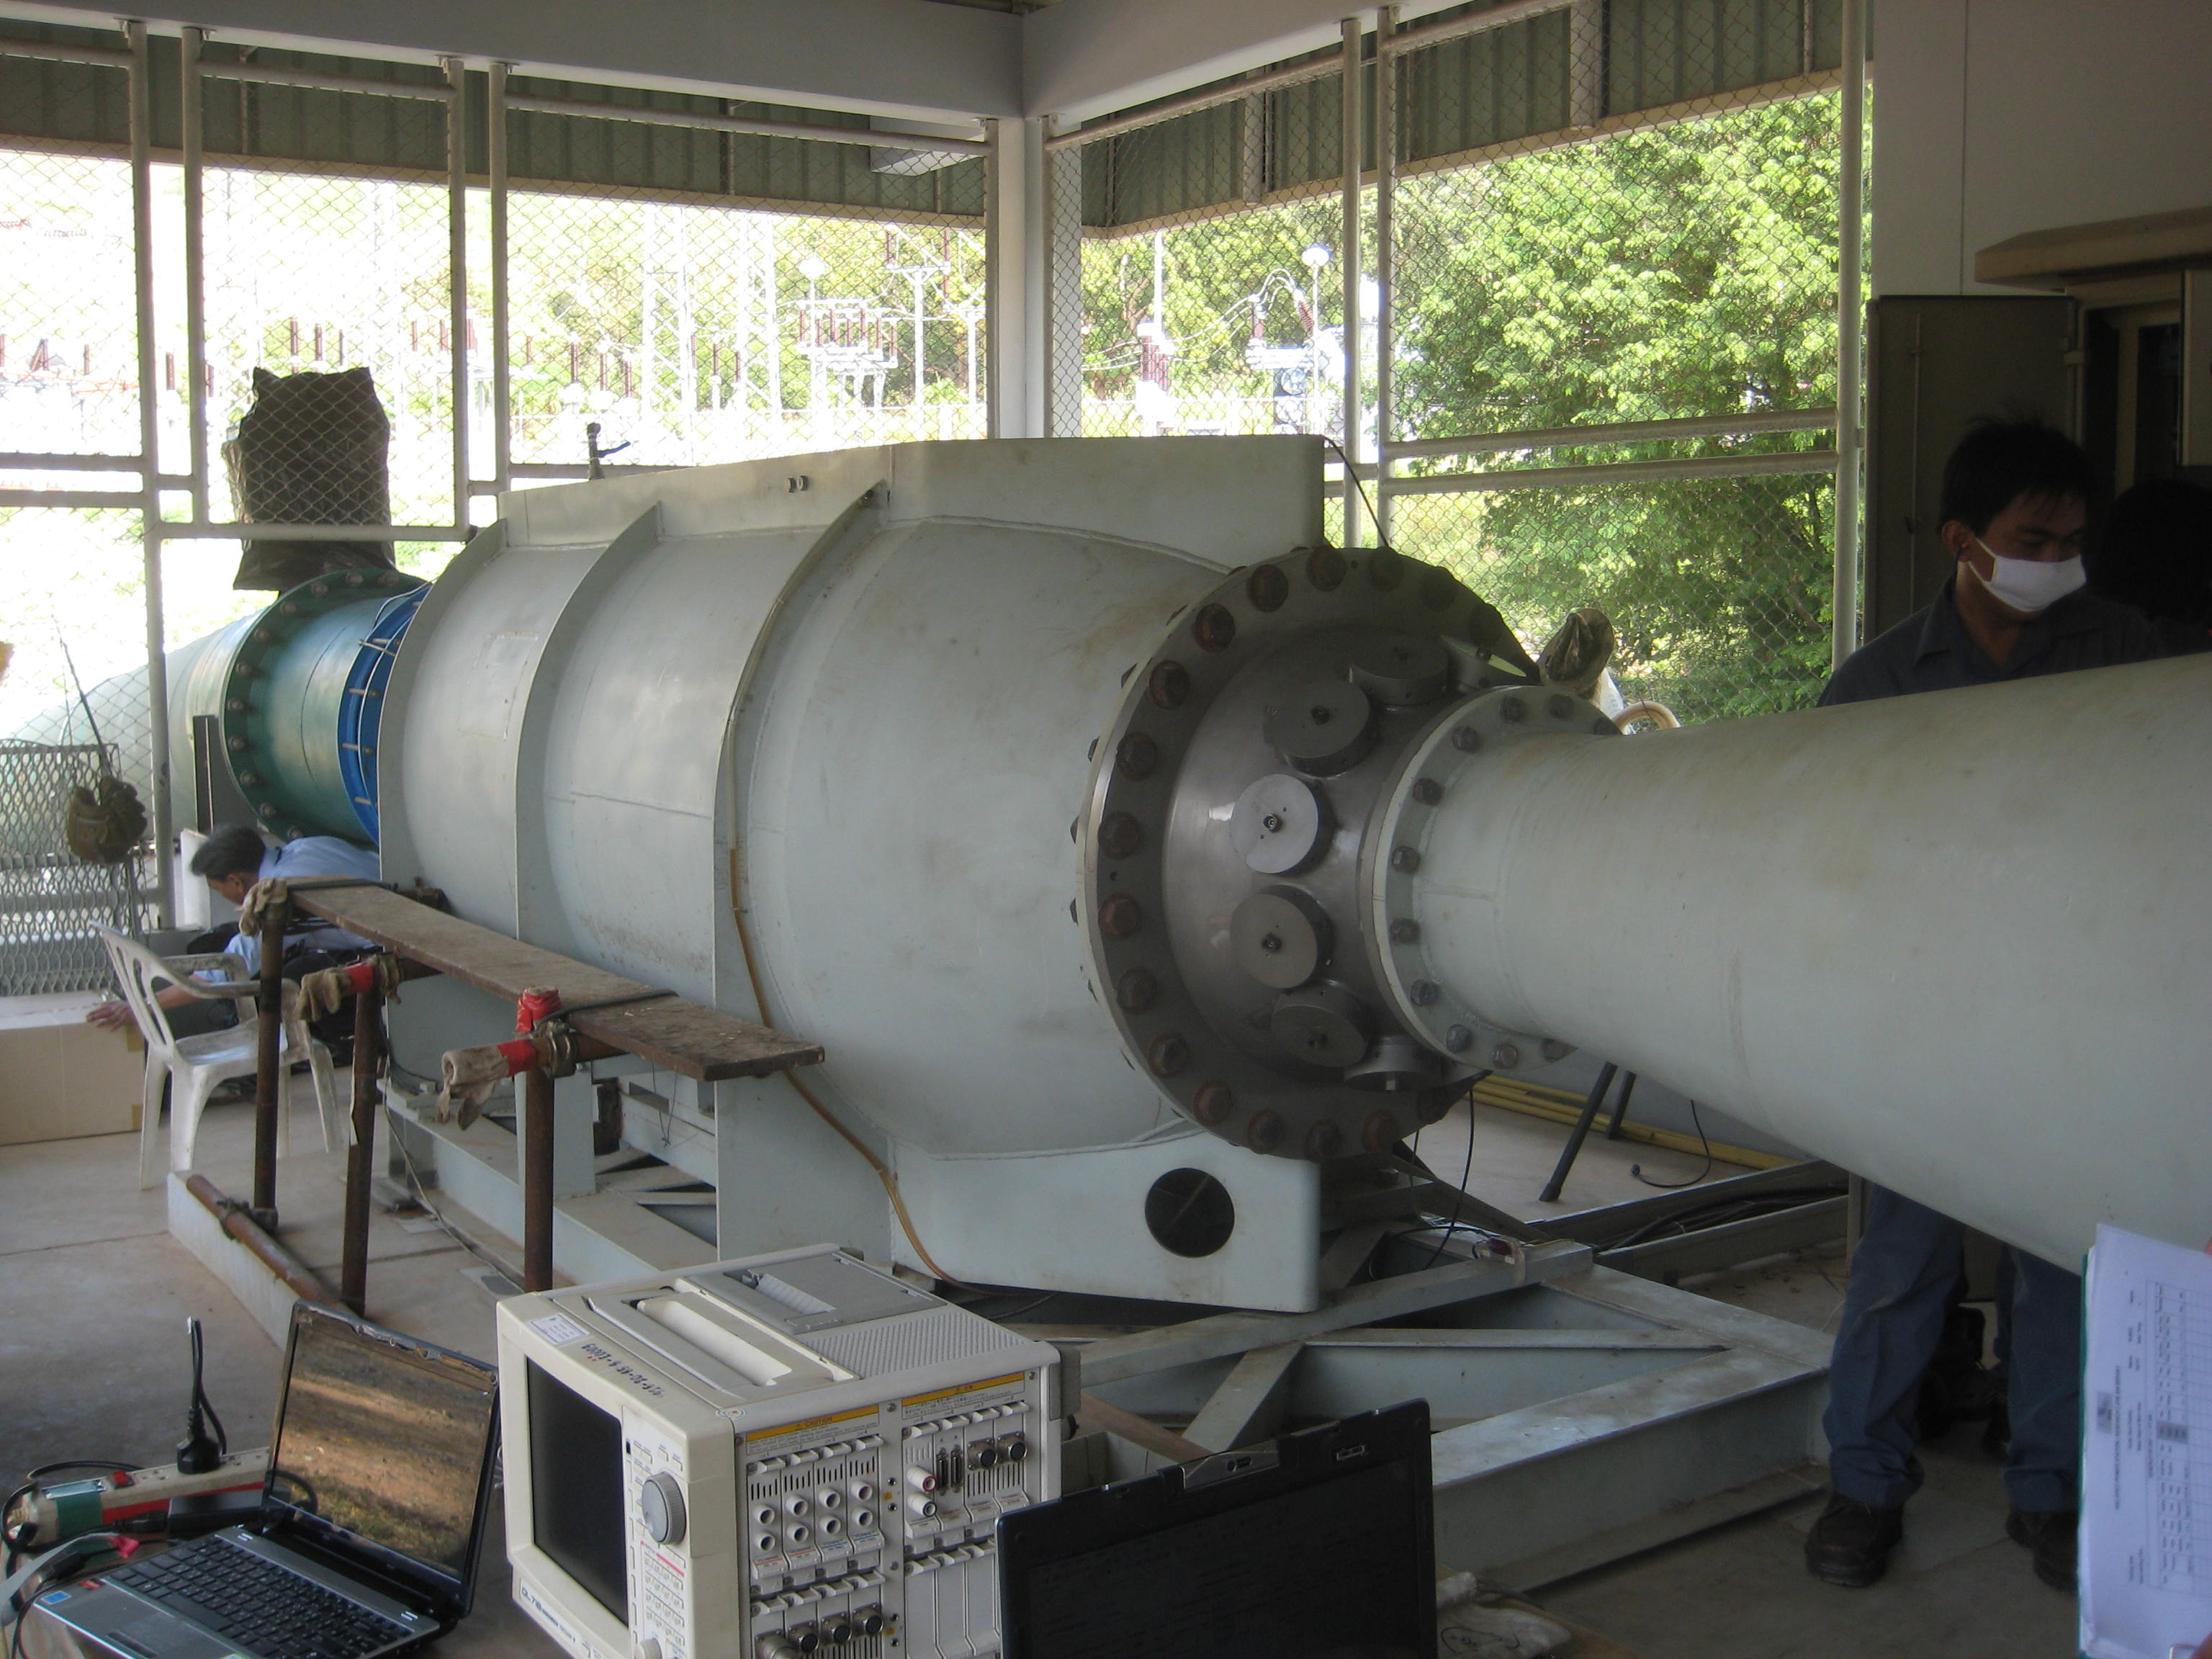
\includegraphics[width=0.82\linewidth]{turbine.JPG}
\caption{The \SI{137}{\kilo\watt} axial-flow bulb turbine installed on the EGAT
performance test rig at the Kaeng Krachan Dam site. Flow enters from the penstock at
right through the bolted-flange casing; the bulb houses the directly coupled induction
generator, and the draft-tube cone extends to the left. At each operating point the
discharge, the generator and mechanical power, and the guide-vane angle were recorded
through the oscilloscope and data-acquisition instrumentation visible in the
foreground. Bringing the rig to a stable condition and averaging repeated readings at
every operating point is the labor-intensive procedure that makes each of the 72
measured points costly and motivates reducing their number.}
\label{fig:rig}
\end{figure}

Performance testing was carried out by EGAT's Power Plant Performance Test Department
(Production Efficiency Division) on a purpose-built rig at the Kaeng Krachan Dam site,
Phetchaburi Province. At each constant head the guide-vane angle was swept while the
discharge and the generator and mechanical power were recorded; the overall (system)
efficiency reported in the dataset is the wire-to-water efficiency, equal to the
turbine mechanical efficiency multiplied by an assumed induction-generator efficiency
of approximately 0.90. The dataset also records the turbine mechanical efficiency
separately. At the BEP both efficiency definitions identify the same operating point,
so the localization analysis that follows is unaffected by the choice between them.
The efficiency magnitudes in this dataset are consistent with the source documentation
once two definitional points are recognized. First, the values analyzed here are
overall system (wire-to-water) efficiencies, whereas the turbine mechanical
efficiencies reported for the same machine are higher: at the BEP the dataset records
an overall efficiency of 0.697 and a mechanical efficiency of 0.777, the ratio being
the assumed generator efficiency of about 0.90. The 78--80\% figures quoted in the
turbine-design literature for this machine family refer to mechanical (turbine)
efficiency, which the present dataset reproduces at 0.777. Second, the source
performance tests computed efficiency from inlet pressure measured at two alternative
planes---before the bulb, and after the bulb just upstream of the guide vanes---giving
maximum turbine efficiencies of 75.17\% (at \SI{17}{\metre} head) and 77.93\% (at
\SI{16}{\metre} head, guide-vane angle \ang{37.5}, discharge
\SI{0.82}{\cubic\metre\per\second}) respectively for this \SI{137}{\kilo\watt} unit.
These are the same measured runs evaluated across different measurement planes, not
different test campaigns, and the \SI{16}{\metre}, \ang{37.5},
\SI{0.82}{\cubic\metre\per\second} peak coincides with the BEP identified in the
present dataset. The dataset analyzed here is therefore the EGAT \SI{137}{\kilo\watt}
small-hydro propeller turbine campaign, with efficiency computed on the after-bulb
plane, the configuration that yields the higher efficiency and whose
mechanical-efficiency peak of 0.777 is consistent with the 77.93\% reported for that
plane. The BEP of the ground-truth dataset lies at
$Q = \SI{0.8185}{\cubic\metre\per\second}$, $H = \SI{16.00}{\metre}$ (guide-vane
angle \ang{37.5}), $\eta^\ast = 0.6973$, which is the point of maximum measured
overall efficiency. We note here, and return to it in Section~\ref{sec:limits}, that
the BEP head coincides exactly with an integer head node of the test matrix; this
coincidence has consequences for the comparison that must be acknowledged.

\subsection{Gaussian-process surrogate and adaptive sampling policies}
The adaptive policy is a Bayesian optimization loop built on a Gaussian process (GP)
surrogate of the efficiency function~\cite{rasmussen2006gpml}, implemented with the
scikit-learn library~\cite{pedregosa2011sklearn}. The GP places a prior over functions
specified by a constant mean and a product covariance kernel,
\begin{equation}
k(\mathbf{x}, \mathbf{x}') = C \cdot k_{\text{Mat\'ern}}(\mathbf{x}, \mathbf{x}';\ \nu = 5/2),
\label{eq:kernel}
\end{equation}
where $C$ is a constant (signal-variance) kernel and $k_{\text{Mat\'ern}}$ is the
Mat\'ern kernel with smoothness parameter $\nu = 5/2$ and a single shared length
scale. The Mat\'ern-5/2 kernel is preferred over the squared-exponential kernel
because it imposes weaker smoothness assumptions appropriate to measured
data~\cite{palar2020compositekernel}. The kernel hyperparameters are obtained by
maximizing the marginal likelihood with five random restarts of the optimizer; a small
jitter ($\alpha = 1\times10^{-6}$) is added to the diagonal for numerical stability,
and the efficiency response is standardized internally. The surrogate takes three
standardized inputs---discharge $Q$, head $H$, and guide-vane angle---and all six
sampling policies use the same three inputs and GP configuration, so the comparison
isolates the sampling strategy alone. The guide-vane angle is the actuated control
variable in this campaign: each $(Q, H)$ condition maps to a unique guide-vane
setting---the within-head Pearson correlation between guide-vane angle and discharge,
averaged over the eight test heads, is 0.986 (range 0.983--0.988)---so an operating
point is fully specified by $(Q, H)$, and the sampling policies operate in the
$(Q, H)$ plane. Reconstruction accuracy is evaluated at all 72 measured operating
points, and the efficiency field is visualized on the conventional $(Q, H)$
hill-chart plane.

Trained on the sampled set $S$ with inputs $X_S$ and measured efficiencies $y_S$,
the Gaussian process yields a posterior at any operating point $\mathbf{x}$ that is
itself Gaussian, with closed-form mean and variance
\begin{align}
\mu_S(\mathbf{x}) &= m + k(\mathbf{x}, X_S)\,[K_S + \sigma_n^2 I]^{-1}(y_S - m),
\label{eq:postmean}\\
\sigma_S^2(\mathbf{x}) &= k(\mathbf{x}, \mathbf{x}) - k(\mathbf{x}, X_S)\,
[K_S + \sigma_n^2 I]^{-1} k(X_S, \mathbf{x}),
\label{eq:postvar}
\end{align}
where $K_S = k(X_S, X_S)$ and $\sigma_n^2$ is the small jitter term. The posterior
mean $\mu_S$ is the reconstructed efficiency surface, while the posterior variance
$\sigma_S^2$ is the surrogate's own admission of how uncertain it remains. Crucially,
the variance in Eq.~\eqref{eq:postvar} depends only on the \emph{locations} of the
observations and not on their measured values, so the informativeness of a candidate
operating point can be scored in closed form before the experiment is run---the
property the active-learning acquisitions exploit.

The three adaptive policies (BO-UCB, ALM, and ALC) share a single greedy loop and
differ only in the acquisition function $a(\mathbf{x})$: (i) initialize $S$ with $n_0$
points drawn at random; (ii) fit the GP on $(X_S, y_S)$ and evaluate $\mu_S$ and
$\sigma_S$ from Eqs.~\eqref{eq:postmean}--\eqref{eq:postvar}; (iii) select
$\mathbf{x}_{\text{next}} = \argmax_{\mathbf{x} \in \mathcal{X}\setminus S}
a(\mathbf{x})$; (iv) run the experiment, append it to $S$, and repeat (ii)--(iv) until
$|S| = n$. The three acquisitions encode different objectives, developed next.

Given the posterior mean $\mu_t(\mathbf{x})$ and posterior standard deviation
$s_t(\mathbf{x})$ after $t$ observations, BO-UCB chooses the next experiment by
maximizing an upper confidence bound acquisition function over the candidate
operating points,
\begin{equation}
a(\mathbf{x}) = \mu_t(\mathbf{x}) + \kappa\, s_t(\mathbf{x}), \qquad \kappa = 2.0.
\label{eq:ucb}
\end{equation}
The upper-confidence-bound criterion is used because it provides an explicit and
interpretable trade-off between exploiting points of high predicted efficiency (the
$\mu$ term) and exploring points of high posterior uncertainty (the $s$ term), with
$\kappa = 2.0$ weighting exploration moderately. At each iteration the GP is refitted
on all points observed so far, the acquisition function is evaluated over all
not-yet-sampled operating points, and the point of maximum acquisition is selected for
the next experiment, which is realized by reading the corresponding ground-truth
efficiency. The loop runs, refitting the surrogate after every observation, until the
experimental budget $n$ is exhausted.

Two Gaussian-process active-learning policies complete the set of adaptive methods.
They share the surrogate, the initialization, and the sequential loop of the Bayesian
policy, and differ only in the acquisition function: whereas the UCB acquisition is
built to find a maximum, the active-learning acquisitions are built to make the
surrogate accurate everywhere, and the contrast between these two design intents is
the methodological axis of the study. Active Learning MacKay (ALM)~\cite{mackay1992alm}
selects the candidate operating point at which the posterior standard deviation is
largest,
\begin{equation}
a(\mathbf{x}) = s_t(\mathbf{x}),
\label{eq:alm}
\end{equation}
so that each experiment removes the largest remaining pocket of predictive
uncertainty. Under a Gaussian process this greedy rule maximizes the information
gained about the function value at the queried point, and it tends to produce a near
space-filling pattern with a mild bias toward the domain boundary, where the posterior
variance is naturally highest. Active Learning Cohn (ALC)~\cite{cohn1996alc} instead
selects the candidate whose observation most reduces the surrogate's integrated
posterior variance over the whole candidate set,
\begin{equation}
a(\mathbf{x}) = -\frac{1}{N}\sum_{i=1}^{N} s^2_{t+\mathbf{x}}(\mathbf{x}_i),
\label{eq:alc}
\end{equation}
where the augmented posterior variance is evaluated at each of the $N$ candidate
points. Because the Gaussian-process posterior variance depends only on the locations
of the observations and not on their measured values, the effect of adding a candidate
can be scored in closed form before the experiment is run, with the fitted kernel held
fixed, at a per-step cost of $O(N)$ candidate evaluations for ALM and UCB and $O(N^2)$
for ALC. ALC is the sequential, greedy counterpart of the integrated-mean-square-error
optimal designs of classical computer-experiment theory~\cite{sacks1989doe}.

\subsection{Initialization}
Every sequential policy (BO-UCB, ALM, and ALC) is initialized with $n_0 = 5$ operating
points drawn uniformly at random, without replacement, from the measured candidate
set, after which the acquisition function governs all subsequent selections. A random
initial design makes the sequential policies stochastic, so their run-to-run
variability is characterized across random seeds on the same footing as the random and
Latin hypercube baselines (Section~\ref{sec:eval}). Structured alternatives, such as
the corners-and-center core of a classical central composite design, are a natural
refinement; a systematic comparison of initialization schemes is identified as future
work in Section~\ref{sec:conclusion}.

\subsection{Baseline design-of-experiments methods}
Three classical, non-adaptive designs serve as baselines, each allocated the same
total experimental budget $n$ as the adaptive policies to ensure a fair comparison.

\emph{Random sampling} draws $n$ operating conditions without replacement from the
measured points. It provides an unbiased but uncontrolled coverage of the space and
serves as the minimal baseline.

\emph{Grid sampling} constructs a regular lattice spanning the discharge and head
ranges and snaps each lattice node to the nearest measured operating point,
reproducing the conventional practice of testing at evenly spaced operating
conditions; when the budget is not a perfect square, the selection is completed to $n$
with randomly chosen unused points, so grid sampling is also mildly stochastic at such
budgets.

\emph{Latin hypercube sampling}~\cite{mckay1979lhs} generates a two-dimensional
space-filling design over the discharge--head ranges with even one-dimensional
stratification, snaps each sample to the nearest measured point, and fills any
shortfall with randomly chosen unused points.

For every design, the sampled conditions are evaluated against the ground-truth
dataset, a surrogate is fitted to the resulting observations using the same Gaussian
process specification as in the preceding subsection to ensure that differences in
performance arise from the sampling policy and not from the interpolating model, and
the fitted surrogate is used both to reconstruct the surface and to estimate the BEP.
All six policies retain a stochastic element---the sequential policies through their
random initialization, grid sampling through its random completion at non-square
budgets, and random and Latin hypercube sampling by construction---and all are
therefore evaluated across random seeds (Section~\ref{sec:eval}).

\subsection{Evaluation protocol}\label{sec:eval}
All policies are evaluated at a series of common budgets $n$ swept from 6 to 30
experiments against the complete measured dataset of 72 points; a budget of $n$
corresponds to a reduction of $(72 - n)/72$ in the number of physical experiments,
from 58.3\% at $n = 30$ to 91.7\% at $n = 6$. The budget $n = 12$ (an 83.3\%
reduction) serves as the headline operating point for the tables and illustrative
figures, chosen by the engineering criterion stated in Section~\ref{sec:budget}.

\emph{Global reconstruction metrics.} The reconstructed surface is compared to the
ground truth over all 72 experimental points using the mean absolute error (MAE), the
root-mean-square error (RMSE), the coefficient of determination ($R^2$), and the mean
absolute percentage error (MAPE). These metrics rank the policies under the
global-reconstruction objective; under the localization objective they are reported
only to characterize each policy's behavior.

\emph{BEP localization metrics.} The primary metrics are the absolute errors in the
predicted BEP location and value relative to ground truth: the discharge error
$|\hat{Q} - Q^\ast|$, the head error $|\hat{H} - H^\ast|$, and the efficiency error
$|\hat{\eta} - \eta^\ast|$. To avoid crediting a policy merely for sampling the peak,
the BEP is read from the GP prediction over the full 72-point grid, not from the
sampled rows.

\emph{Statistical protocol.} Because every policy retains a stochastic element, all
metrics are computed across 20 independent random seeds and reported as mean
$\pm$ standard error; each seed fixes the random initialization of the sequential
policies and the draws of the random and Latin hypercube designs. Pairwise
differences between policies are tested with one-sided Wilcoxon signed-rank tests,
pairing the methods on the seeds as matched replications; with 20 seeds the smallest
attainable exact $p$-value is $2^{-20} \approx 10^{-6}$.

\emph{Budget analysis.} To quantify the achievable experiment reduction, both the
global reconstruction error and the BEP localization error are reported as functions
of the budget $n$ over the range 6 to 30 experiments, and the smallest budget at which
the Bayesian policy locates the exact BEP node on every seed is determined.

%======================================================================
\section{Results}\label{sec:results}
%======================================================================
The results are organized around the two objectives defined in
Section~\ref{sec:problem}. Section~\ref{sec:recon} reports global hill-chart
reconstruction; Section~\ref{sec:local} reports best-efficiency-point localization;
Section~\ref{sec:budget} presents the budget sweep that is the core evidence of the
study; Section~\ref{sec:sig} gives the significance tests; Section~\ref{sec:lowbudget}
examines the very-low-budget regime; Section~\ref{sec:uncertainty} verifies that the
surrogate's posterior uncertainty tracks its actual error; and
Section~\ref{sec:guidance} distills the findings into practical guidance for planning a
reduced test campaign. All policies are
averaged over 20 seeds and reported as mean $\pm$ standard error. Unless stated
otherwise the illustrative budget is $n = 12$, an 83.3\% reduction from the 72-point
campaign (justified in Section~\ref{sec:budget}).

\subsection{Global hill-chart reconstruction}\label{sec:recon}
For recovering the entire efficiency map, the model-based active learners are the
strongest methods and the optimizer is the weakest. Table~\ref{tab:metrics} reports
reconstruction and localization metrics for all six policies at $n = 12$. The
integrated-variance active learner ALC attains the best global accuracy
($R^2 = 0.9965$, $\mathrm{MAE} = 0.00218$, $\mathrm{MAPE} = 0.35\%$), with the
maximum-variance learner ALM statistically indistinguishable from it ($R^2 = 0.9961$;
the difference is not significant, Section~\ref{sec:sig}). The space-filling designs
follow (LHS $R^2 = 0.9945$, grid $R^2 = 0.9938$), while random sampling
($R^2 = 0.9380$) and, notably, Bayesian optimization ($R^2 = 0.9207$) are markedly
worse. BO-UCB is the worst map-builder of the six: by design it concentrates its
budget near the predicted optimum and starves the rest of the domain, so its surrogate
is accurate near the peak but biased elsewhere---the expected behavior of an
optimization acquisition applied to a reconstruction task.
Fig.~\ref{fig:allmethods2d} shows the reconstructed hill chart obtained by each of the
six policies at $n = 12$, and Fig.~\ref{fig:allmethods3d} presents the same
reconstructions as three-dimensional efficiency surfaces at a shared viewing angle.
Fig.~\ref{fig:allmethodserr} maps the absolute reconstruction error for each policy
over the operating plane, and Fig.~\ref{fig:allmethodserr3d} presents the same error
as three-dimensional surfaces, on which the tall error ridge over the low-efficiency,
high-discharge corner produced by random sampling and BO-UCB is immediately visible.
Fig.~\ref{fig:placement} then contrasts where each policy places its 12 experiments.
Across these views the active learners and space-filling designs cover the whole
envelope, whereas BO-UCB leaves the low-efficiency, high-discharge corner sparse and
reconstructs it poorly.

\begin{table}[t]
\centering
\caption{Reconstruction and BEP-localization metrics at $n = 12$ (83.3\% reduction),
mean over 20 seeds. Best value in each column in bold. Reconstruction: lower
MAE/RMSE/MAPE and higher $R^2$ are better. Localization: lower
$\Delta Q/\Delta H/\Delta\eta$ are better.}
\label{tab:metrics}
\small
\begin{tabular}{@{}lccccccc@{}}
\toprule
Method & MAE & RMSE & $R^2$ & MAPE (\%) & $\Delta Q$ & $\Delta H$ & $\Delta\eta$ \\
\midrule
ALC    & \textbf{0.00218} & \textbf{0.00354} & \textbf{0.9965} & \textbf{0.35} & 0.0235 & 0.50 & 0.00714 \\
ALM    & 0.00239 & 0.00380 & 0.9961 & 0.38 & 0.0131 & 0.75 & 0.01015 \\
LHS    & 0.00272 & 0.00445 & 0.9945 & 0.44 & 0.0215 & 0.80 & 0.00748 \\
Grid   & 0.00313 & 0.00476 & 0.9938 & 0.50 & \textbf{0.0108} & 0.70 & 0.01131 \\
Random & 0.00609 & 0.00988 & 0.9380 & 1.07 & 0.0230 & 0.55 & 0.00861 \\
BO-UCB & 0.00986 & 0.01577 & 0.9207 & 1.77 & 0.0137 & \textbf{0.00} & \textbf{0.00030} \\
\bottomrule
\end{tabular}
\end{table}

\begin{figure}[t]
\centering
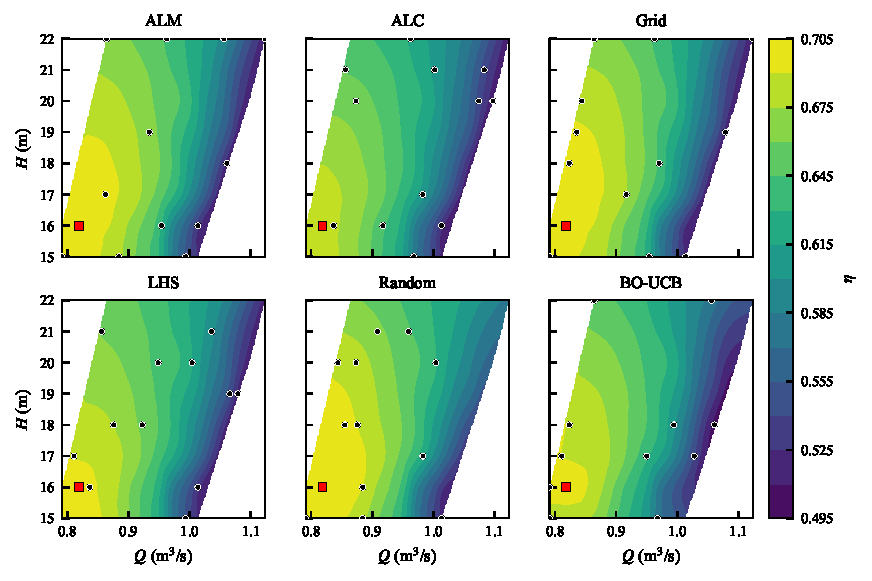
\includegraphics[width=\linewidth]{fig_all_methods_2d.pdf}
\caption{Reconstructed hill-chart contours at $n = 12$ for all six policies (the 12
sampled points in black, the true BEP marked by a red square). The active learners and
space-filling designs recover the whole surface, whereas BO-UCB distorts the
low-efficiency, high-discharge region.}
\label{fig:allmethods2d}
\end{figure}

\begin{figure}[t]
\centering
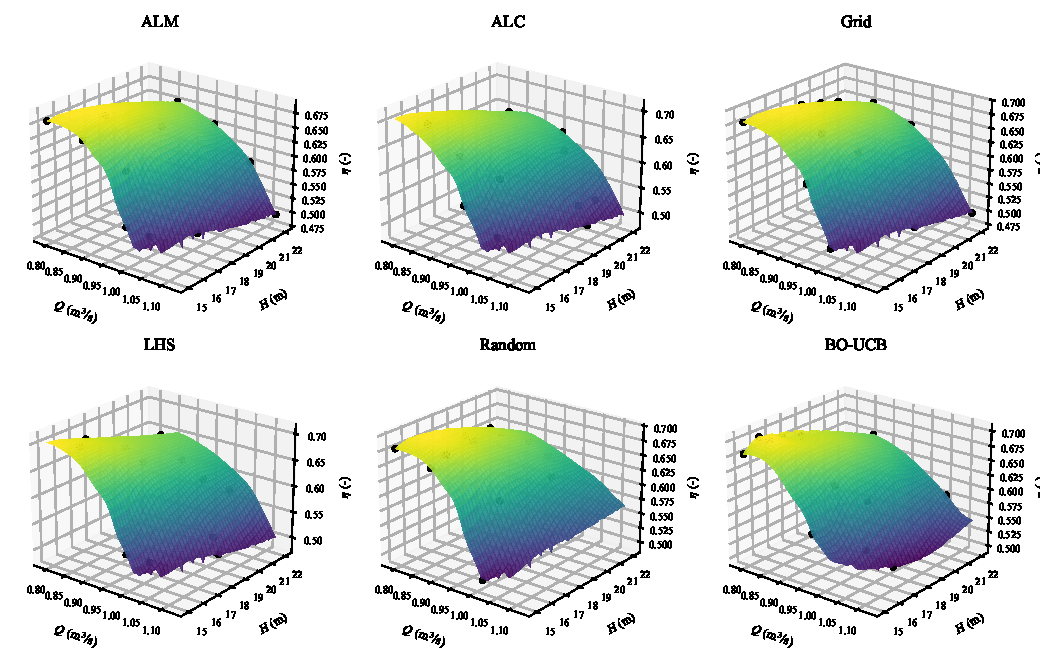
\includegraphics[width=\linewidth]{fig_all_methods_3d.pdf}
\caption{Reconstructed efficiency surfaces at $n = 12$ for all six policies, rendered
at the shared viewing angle used throughout for comparability. Sampled points are
shown in black.}
\label{fig:allmethods3d}
\end{figure}

\begin{figure}[t]
\centering
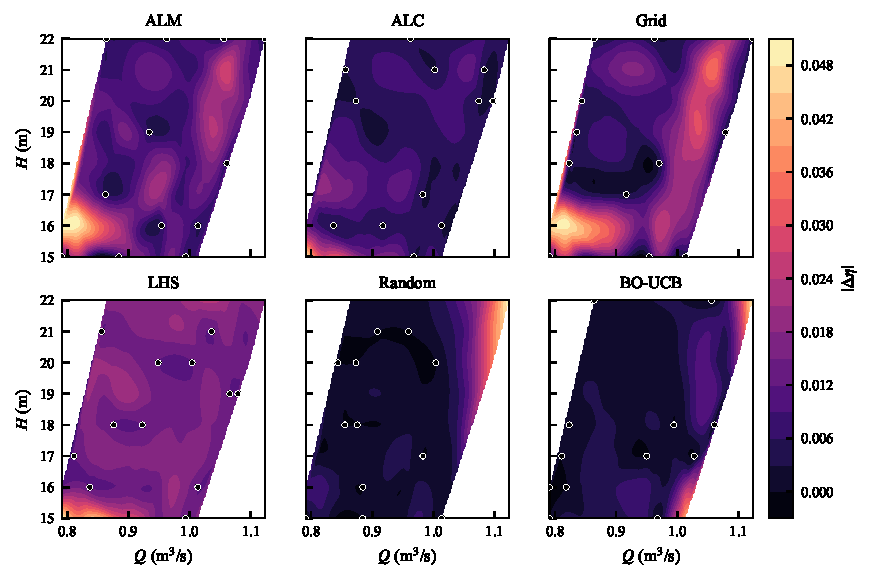
\includegraphics[width=\linewidth]{fig_all_methods_error.pdf}
\caption{Absolute reconstruction error $|\Delta\eta|$ at $n = 12$ for all six
policies. The error concentrates where a policy leaves the operating envelope sparsely
sampled.}
\label{fig:allmethodserr}
\end{figure}

\begin{figure}[t]
\centering
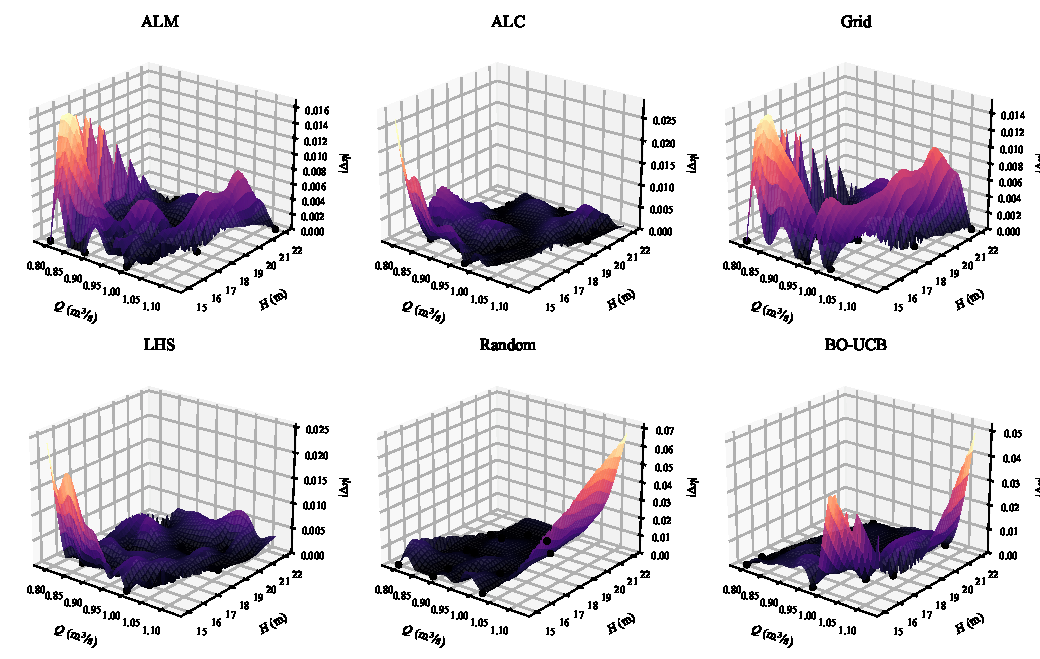
\includegraphics[width=\linewidth]{fig_all_methods_error_3d.pdf}
\caption{Absolute reconstruction error $|\Delta\eta|$ at $n = 12$ for all six policies
as three-dimensional surfaces (the companion to Fig.~\ref{fig:allmethodserr}). The
vertical scale exposes how much larger the peak error is for random sampling and
BO-UCB---a tall ridge over the low-efficiency, high-discharge corner---than for the
active learners and space-filling designs.}
\label{fig:allmethodserr3d}
\end{figure}

\begin{figure}[t]
\centering
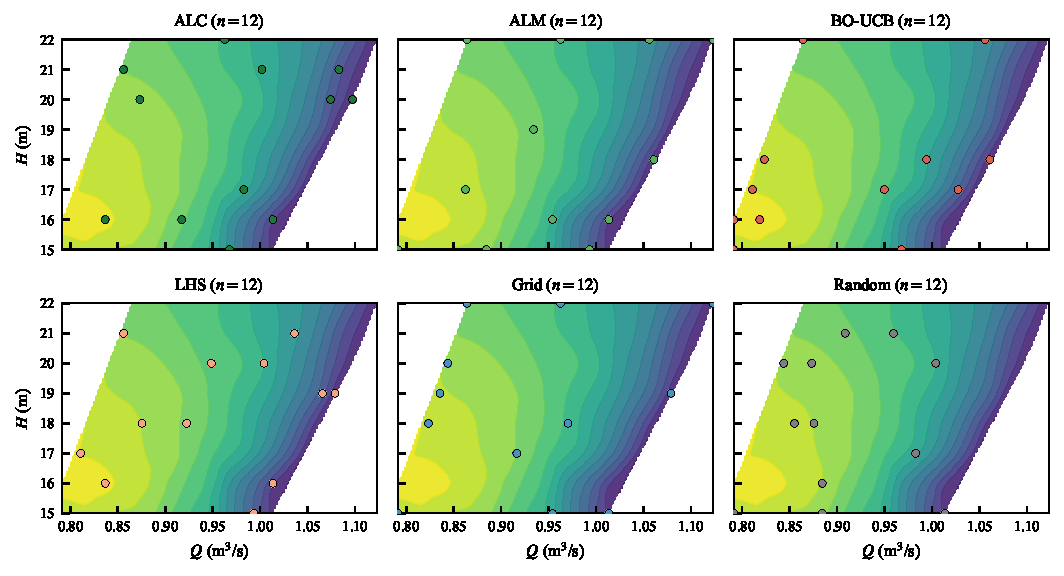
\includegraphics[width=\linewidth]{fig_sample_placement.pdf}
\caption{Sample placement at $n = 12$ for all six policies over the ground-truth
efficiency contour: the active learners and space-filling designs cover the envelope,
whereas BO-UCB concentrates on the high-efficiency ridge.}
\label{fig:placement}
\end{figure}

\subsection{Best-efficiency-point localization}\label{sec:local}
For the opposite objective---pinpointing the BEP---the ranking inverts. The rightmost
columns of Table~\ref{tab:metrics} report the localization errors, and here Bayesian
optimization is decisively best: at $n = 12$ it already matches the ground-truth head
exactly ($\Delta H = 0$) and reaches an efficiency error $\Delta\eta = 0.0003$, one to
two orders of magnitude below every other method ($\Delta\eta$ between 0.007 and 0.011
for the active learners and space-filling designs). By $n = 14$ the UCB policy locates
the exact BEP node, with discharge, head, and efficiency error all at the level of
numerical noise ($\Delta\eta \to 0$). This follows directly from the exploitation term
of the UCB acquisition: it climbs the efficiency ridge and expends its budget resolving
the peak---exactly what BEP localization rewards and exactly what penalized it on the
global metric. The active learners and space-filling designs, spreading their budget
for coverage, never resolve the optimum as sharply and plateau near $10^{-2}$.
Fig.~\ref{fig:contrast} juxtaposes the two behaviors at the same budget in a single
frame.

\begin{figure}[t]
\centering
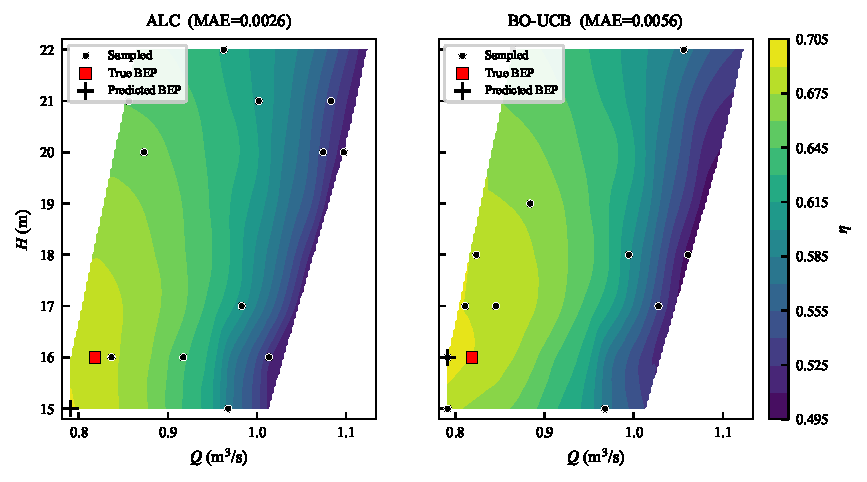
\includegraphics[width=\linewidth]{fig_goal_contrast.pdf}
\caption{The two goals in one frame: ALC (left) and BO-UCB (right) at the same budget
$n = 12$. BO-UCB pins the BEP but distorts the map; ALC recovers the map but locates
the BEP less precisely. This contrast is the thesis of the paper: the acquisition
function must match the deliverable.}
\label{fig:contrast}
\end{figure}

\subsection{Experiment budget versus accuracy}\label{sec:budget}
The central evidence of the study is the budget sweep in Fig.~\ref{fig:curves}, which
reports both objectives as a function of the number of experiments $n$ from 6 to 30.
For reconstruction (panel a) the active learners reach engineering-grade accuracy very
early: ALC attains $R^2 = 0.994$ by $n = 10$ and $R^2 = 0.996$ by $n = 12$, and ALM
tracks it closely, while BO-UCB never exceeds $R^2 \approx 0.96$ anywhere in the range.
For localization (panel b) BO-UCB drives the BEP efficiency error to 0.0003 by
$n = 12$ and to the level of numerical noise (below $4\times10^{-6}$) by $n = 14$,
whereas the other methods remain near $10^{-2}$ throughout. At large budgets
($n \geq 25$) all reconstruction methods saturate above $R^2 = 0.99$ and the
differences vanish; the value of the comparison is visible only in the low-budget
regime, which is precisely where experiments are scarce.

\begin{figure}[t]
\centering
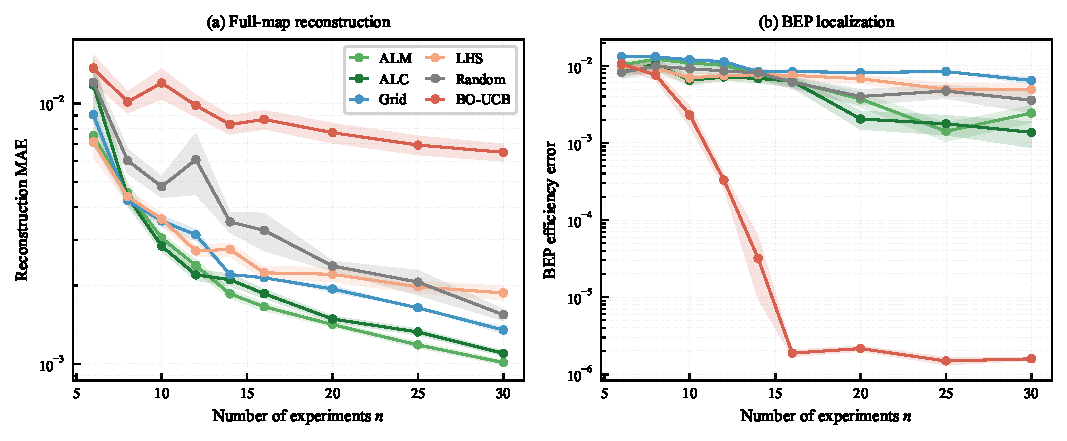
\includegraphics[width=\linewidth]{fig_learning_curves.pdf}
\caption{Learning curves over the budget sweep (mean $\pm$ standard error, 20 seeds).
(a) Global reconstruction versus $n$: the active learners (ALC, ALM) dominate and
BO-UCB is worst. (b) BEP efficiency error versus $n$: BO-UCB dominates, reaching the
level of numerical noise by $n = 14$, while the others plateau. The inversion between
the panels is the core result.}
\label{fig:curves}
\end{figure}

This motivates $n = 12$ as the headline budget for the illustrative figures, chosen by
an explicit engineering criterion---the smallest budget at which the recommended
reconstruction method reaches $R^2 \geq 0.99$ and $\mathrm{MAPE} < 0.5\%$---rather than
by inspection. ALC clears this bar at $n = 10$ ($R^2 = 0.994$, $\mathrm{MAPE} = 0.46\%$)
and ALM at $n = 12$ ($R^2 = 0.996$, $\mathrm{MAPE} = 0.38\%$); we adopt $n = 12$, the
conservative point at which both recommended learners clear the bar, an 83.3\%
reduction from the full campaign.

The headline reduction result follows directly. For the full hill chart, active
learning attains $R^2 \approx 0.996$ from just 12 of the 72 measured points---an 83\%
reduction---and reaches $R^2 \geq 0.99$ from as few as 10 points. For the BEP alone,
Bayesian optimization identifies the exact optimum node using 14 experiments, an 81\%
reduction. In both cases the deliverable is obtained at well under a quarter of the
original test effort, provided the sampling policy is matched to the objective.

\subsection{Statistical significance}\label{sec:sig}
Because these averages could reflect seed-to-seed luck, each headline claim is tested
with a Wilcoxon signed-rank test, pairing methods on the 20 seeds as matched
replications (Table~\ref{tab:wilcoxon}). For reconstruction (reference ALC at
$n = 12$) ALC significantly outperforms BO-UCB ($p \approx 10^{-6}$), random
($p \approx 10^{-5}$), grid ($p = 1.3\times10^{-4}$) and LHS ($p = 0.009$), while the
ALC--ALM difference is not significant ($p = 0.09$): the two active learners are
statistically equivalent. For localization (reference BO-UCB at $n = 12$) BO-UCB beats
every other method on efficiency error at $p \leq 4.8\times10^{-6}$, at or near the
smallest $p$ attainable with 20 seeds, a floor small enough that its localization
advantage is unambiguous. Read across budgets, ALC and ALM significantly beat BO-UCB
and random at essentially every $n \geq 8$ and beat grid and LHS from $n = 12$ upward;
the ALM--ALC difference is never significant, so we recommend ALM as the practical
default for reconstruction---equal accuracy at lower computational cost.
Fig.~\ref{fig:bars} visualizes the ranking inversion between the two objectives at
$n = 12$.

\begin{table}[t]
\centering
\caption{Wilcoxon signed-rank tests at $n = 12$ (20 seeds, paired by seed). Top:
reconstruction MAE, reference ALC. Bottom: BEP efficiency error, reference BO-UCB.
$p < 0.05$ is significant.}
\label{tab:wilcoxon}
\small
\begin{tabular}{@{}llcc@{}}
\toprule
Comparison & Metric & $p$-value & Significant? \\
\midrule
ALC vs.\ ALM     & MAE & 0.09 & no (equivalent) \\
ALC vs.\ LHS     & MAE & 0.009 & yes \\
ALC vs.\ Grid    & MAE & $1.3\times10^{-4}$ & yes \\
ALC vs.\ Random  & MAE & $1.3\times10^{-5}$ & yes \\
ALC vs.\ BO-UCB  & MAE & $9.5\times10^{-7}$ & yes \\
\midrule
BO-UCB vs.\ ALC    & $\Delta\eta$ & $9.5\times10^{-7}$ & yes \\
BO-UCB vs.\ ALM    & $\Delta\eta$ & $9.5\times10^{-7}$ & yes \\
BO-UCB vs.\ LHS    & $\Delta\eta$ & $4.8\times10^{-6}$ & yes \\
BO-UCB vs.\ Grid   & $\Delta\eta$ & $9.5\times10^{-7}$ & yes \\
BO-UCB vs.\ Random & $\Delta\eta$ & $9.5\times10^{-7}$ & yes \\
\bottomrule
\end{tabular}
\end{table}

\begin{figure}[t]
\centering
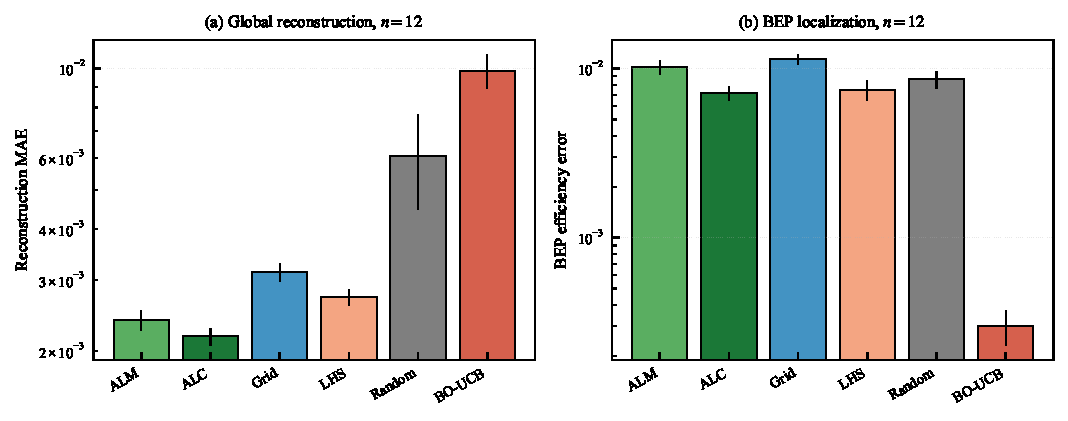
\includegraphics[width=\linewidth]{fig_metrics_bars.pdf}
\caption{Method ranking at $n = 12$ with standard-error bars. (a) Reconstruction:
active learners best. (b) BEP localization: BO-UCB best. The ranking inverts between
the two objectives.}
\label{fig:bars}
\end{figure}

\subsection{The very-low-budget regime}\label{sec:lowbudget}
One qualification bounds the recommendation. Below about eight experiments the Gaussian
process is fitted on too few points for the model-based acquisitions to be reliable,
and the integrated-variance learner in particular can degrade: at $n = 6$, ALC drops
to $R^2 = 0.82$ and BO-UCB to $R^2 = 0.84$, whereas the space-filling and
maximum-variance designs remain robust (LHS $R^2 = 0.97$, grid $R^2 = 0.96$, ALM
$R^2 = 0.97$). In this extreme-reduction corner a model-free space-filling design is
the safer choice. The practical guidance is therefore tiered: use Latin hypercube
sampling for the smallest budgets ($n < 8$) and switch to active learning (ALM or ALC)
once $n \geq 10$, where it reliably dominates. For BEP localization the recommendation
is unqualified across the range examined: Bayesian optimization is preferred at every
budget.

In summary, the six policies separate cleanly into three groups matched to purpose:
the active learners (ALC, ALM) for reconstructing the whole hill chart, Bayesian
optimization for locating the BEP, and space-filling designs (chiefly LHS) as the
robust fallback at the very lowest budgets. Both recommended tools are data-driven and
share the same surrogate, so the practical cost of choosing the sampler to match the
objective is negligible.

\subsection{Posterior uncertainty as a stopping signal}\label{sec:uncertainty}
The adaptive stopping rule discussed in Section~\ref{sec:decision} is viable only if
the surrogate's own uncertainty is informative about its actual error.
Fig.~\ref{fig:uncert} compares the Gaussian-process posterior standard deviation
$\sigma$ with the absolute reconstruction error $|\Delta\eta|$ for the ALC design at
$n = 12$ (seed 0). The two fields share the same spatial structure: both attain their
largest values in the sparsely sampled low-discharge, low-head corner of the envelope
and both are small throughout the well-covered interior. The agreement is quantitative
as well as visual, with a Pearson correlation of $r = 0.70$ between $\sigma$ and
$|\Delta\eta|$ at the 72 measured points ($p < 10^{-11}$). The posterior uncertainty
is therefore a usable running proxy for where, and by how much, the reconstruction
remains untrustworthy, which is precisely the property an uncertainty-based stopping
criterion relies on.

\begin{figure}[t]
\centering
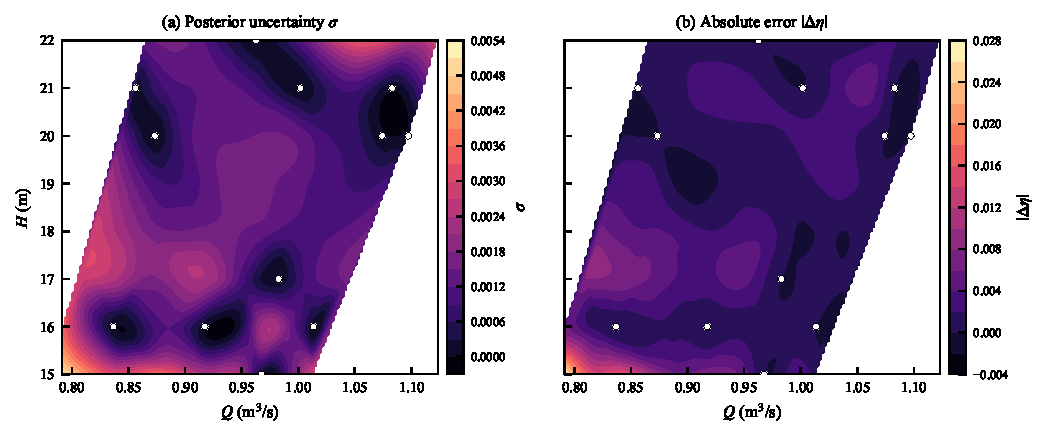
\includegraphics[width=\linewidth]{fig_uncertainty.pdf}
\caption{Gaussian-process posterior uncertainty $\sigma$ (a) and absolute
reconstruction error $|\Delta\eta|$ (b) for the ALC design at $n = 12$ (seed 0), with
the 12 sampled points marked. The two fields are strongly correlated (Pearson
$r = 0.70$ at the 72 measured points), supporting the use of posterior uncertainty as
a stopping signal.}
\label{fig:uncert}
\end{figure}

\subsection{Practical guidance: choosing the budget and the sampler}\label{sec:guidance}
The preceding results translate into a compact recipe that an engineer can apply
before a campaign begins, summarized in Table~\ref{tab:guidance}. The decision has two
inputs: the deliverable (the full hill chart or only the BEP) and the budget the
campaign can afford. For the common deliverable---the full hill chart---the sweet spot
is $n = 10$ to $12$ experiments, an 86\% to 83\% reduction from the 72-point campaign.
This is the smallest budget at which the active learners reach engineering-grade
accuracy ($R^2 \geq 0.99$, $\mathrm{MAPE} < 0.5\%$) while remaining clear of the
$n < 8$ regime in which the Gaussian process is fitted on too few points to be
reliable (Section~\ref{sec:lowbudget}); we recommend $n = 12$ as the conservative
default and $n = 10$ when experiments are especially scarce. Below eight experiments,
where a model-based policy cannot yet be trusted, a space-filling Latin hypercube
design is the safer choice and still recovers the surface to $R^2 \approx 0.97$ at an
89\% to 92\% reduction. If the deliverable is only the BEP, 14 experiments (an 81\%
reduction) with BO-UCB are sufficient to locate the exact optimum node. Because ALM
and ALC are statistically indistinguishable for reconstruction
(Section~\ref{sec:sig}), we recommend ALM as the default reconstruction sampler on the
grounds of lower computational cost. Two caveats travel with the table: the budgets
are calibrated on a smooth, unimodal low-head propeller hill chart and should be
revisited for machines with more structured efficiency surfaces, and the very-low-
budget recommendation assumes the practitioner cannot afford the space-filling
initialization that would stabilize a model-based policy.

\begin{table}[t]
\centering
\caption{Practical guidance for a reduced test campaign on a smooth low-head
propeller hill chart. Reduction is relative to the 72-point reference campaign;
accuracy figures are the mean over 20 seeds.}
\label{tab:guidance}
\small
\begin{tabular}{@{}p{3.1cm}p{2.1cm}ccp{3.4cm}@{}}
\toprule
Deliverable & Recommended sampler & Budget $n$ & Reduction & Expected accuracy \\
\midrule
Full hill chart (default) & ALM (or ALC) & 12 & 83\% & $R^2 \approx 0.996$, MAPE $0.38\%$ \\
Full hill chart (aggressive) & ALC & 10 & 86\% & $R^2 \approx 0.99$, MAPE $< 0.5\%$ \\
Full hill chart (extreme, model-free) & LHS & 6--8 & 89--92\% & $R^2 \approx 0.97$ \\
Best efficiency point only & BO-UCB & 14 & 81\% & exact BEP node, $\Delta\eta \to 0$ \\
\bottomrule
\end{tabular}
\end{table}

%======================================================================
\section{Discussion and Conclusion}\label{sec:discussion}
%======================================================================

\subsection{Interpreting the exploitation advantage}
The central finding of this study is that the policy ranked worst by global
surface-reconstruction metrics is the best for locating the best efficiency point, and
that this is not a contradiction but a direct and predictable consequence of how an
exploitation-driven adaptive policy allocates a limited budget. Bayesian optimization
with an upper-confidence-bound criterion concentrates experiments near the apparent
optimum and along the high-efficiency ridge, and declines to sample the
low-efficiency, high-discharge corner (Fig.~\ref{fig:placement}). That corner is
therefore reconstructed poorly, which inflates global error statistics, while the peak
region is resolved essentially exactly, which is what the localization metrics reward:
from 14 experiments the policy identifies the exact BEP node on every seed. The active
learners exhibit the mirror-image behavior: by directing their budget at the
surrogate's remaining uncertainty they reconstruct the whole surface accurately,
including the parts of it that no operator cares about, but they never place enough
experiments at the peak to resolve the optimum sharply, and their localization error
plateaus near $10^{-2}$. The methodological lesson is that the success criterion must
match the decision objective. A study that adopts the global coefficient of
determination as its headline metric will rank the active learners and space-filling
designs first and dismiss the adaptive optimizer, and will thereby recommend a test
plan optimized for a goal---uniform global fidelity---that a BEP-directed engineer did
not actually have. When the goal is BEP identification, the appropriate criteria are
localization accuracy and reliability, and under those criteria the optimization policy
is decisively preferred. This realignment of metric to objective, rather than any
single numerical result, is the contribution most likely to transfer to other turbine
performance-testing campaigns.

\subsection{Decision-support implications}\label{sec:decision}
Framing performance testing as sequential decision-making yields a practical benefit
beyond the choice of sampling policy. Because the Gaussian process surrogate reports a
posterior uncertainty that demonstrably tracks the actual reconstruction error
(Section~\ref{sec:uncertainty}, Fig.~\ref{fig:uncert}), it provides the engineer with
a running estimate of confidence in the current map and, in particular, in the
estimated BEP. This supports an adaptive stopping rule: testing can continue until the
posterior uncertainty in the high-efficiency region, or the acquisition value
available from a further experiment, falls below a threshold the engineer is willing to
accept, rather than until a pre-committed number of points has been measured. The
budget sweep suggests that such a rule would have terminated testing at roughly 14
experiments for a BEP-directed campaign on the present machine, and at 10 to 12
experiments for hill-chart reconstruction, against the 72 of the full campaign. The
non-adaptive designs cannot support such a rule, because they do not use the observed
efficiencies to guide sampling: their sample locations are fixed before any data are
seen and cannot respond to where the surrogate remains most uncertain. In a setting
where each experiment is genuinely expensive, the ability to decide when to stop on a
principled basis is as valuable as the ability to decide where to test next, and both
follow from the decision-theoretic framing adopted here.

\subsection{Limitations}\label{sec:limits}
Several limitations bound the conclusions of this study. First, the ground-truth BEP
head coincides exactly with an integer head node of the test matrix. This coincidence
favors any policy that samples that node and contributes to the exact BEP recovery
reported for the Bayesian policy; a perturbation analysis in which the BEP is defined
on a continuous interpolant, or in which the test grid is offset, would establish how
much of the localization advantage survives when the optimum does not lie on a node.
Second, the near-zero localization error of the Bayesian policy reflects direct
measurement of the peak region rather than superior out-of-sample interpolation there:
the policy spends its budget inside the high-efficiency envelope, and its advantage
should be understood accordingly. Third, all sequential policies are initialized at
random, and below about eight experiments the Gaussian process is fitted on too few
points for the model-based acquisitions to be reliable (Section~\ref{sec:lowbudget});
a structured initialization, such as the corners-and-center core of a central
composite design, might improve this very-low-budget behavior and remains to be
compared systematically. Fourth, the study concerns one machine and one measured
dataset, so the generality of the finding across other propeller turbines, other
turbine types, and other operating envelopes is not established. None of these
limitations undermines the qualitative finding, but each constrains how strongly it can
be stated.

\subsection{Conclusion and future work}\label{sec:conclusion}
This paper has formulated the construction of a small-hydro propeller-turbine
performance map from physical experiments as a sequential, budget-constrained decision
problem, and has benchmarked six sampling policies---Bayesian optimization, two
Gaussian-process active-learning policies, and random, grid, and Latin hypercube
designs---on a measured ground-truth dataset of 72 points, with the best efficiency
point as an explicit decision target. The study finds that the two engineering
objectives select opposite winners. For reconstructing the full hill chart, the active
learners dominate, reaching $R^2 \geq 0.99$ from as few as 10 experiments and
$R^2 \approx 0.996$ from 12 (an 83.3\% reduction), while the optimization policy is the
weakest map-builder. For locating the BEP the ranking inverts: Bayesian optimization
identifies the exact BEP node on every seed from 14 experiments (an 81\% reduction),
while every other policy plateaus near $\Delta\eta \approx 10^{-2}$. The practical
implication is that turbine performance testing should be planned as a targeted
decision process whose sampling policy---and whose success metric---matches the
deliverable: active learning when the deliverable is the hill chart, Bayesian
optimization when it is the BEP, and a space-filling design as the robust fallback at
the very smallest budgets. For the practitioner these findings reduce to a concrete
budget recipe (Table~\ref{tab:guidance}): the hill chart is recovered at the sweet
spot of 10 to 12 experiments (an 83\% to 86\% reduction) and the BEP at 14 experiments
(an 81\% reduction), with Latin hypercube sampling as the safe choice below eight
experiments. Although demonstrated on a single small-hydro propeller turbine, the sequential-decision framing is not specific to this machine:
objective-directed adaptive sampling has been applied to the optimization of other
small-scale energy-conversion devices~\cite{sefidgar2023crossflow}, and the present
results suggest that comparable budget savings should transfer to any expensive
performance-mapping campaign in which the deliverable is well defined.

Future work should test the sensitivity of the result to the placement of the BEP
relative to the test grid, compare structured initialization schemes against the
random initialization used here, examine the robustness of the ranking to the choice
of GP kernel, and extend the comparison to a second measured dataset, other turbine
types, and other operating envelopes. Incorporating additional decision
objectives---such as the joint consideration of efficiency and cavitation
margin---within the same sequential-decision framework, and integrating a principled
stopping rule based on posterior uncertainty into a live test campaign, are promising
directions for reducing the cost of turbine performance characterization in practice.

%======================================================================
\section*{Acknowledgements}
%======================================================================
The authors gratefully acknowledge the Electricity Generating Authority of Thailand
(EGAT), and in particular its Power Plant Performance Test Department, for conducting
the propeller-turbine performance tests at the Kaeng Krachan site and for making the
resulting experimental data available for this study. The authors also thank Kasetsart
University, Sriracha Campus, and Rambhai Barni Rajabhat University for their
institutional and technical support throughout the work.

\section*{Conflict of Interest}
The authors declare that they have no known competing financial interests or personal
relationships that could have appeared to influence the work reported in this paper.

\section*{Declaration of generative AI in scientific writing}
During the preparation of this work, the authors used Claude (Anthropic) as a coding
assistant to implement the analysis pipeline, generate the figures, and refine the
language of the manuscript. The research idea, problem formulation, methodology, and
all interpretations and conclusions are the authors' own. Every AI-assisted output was
reviewed, verified, and edited by the authors, who take full responsibility for the
content and integrity of the work.

\section*{CRediT Author Contribution Statement}
\textbf{Siwakorn Suprasertchai:} Conceptualization, Methodology, Software, Validation,
Visualization, Project administration. \textbf{Kornpaphop Ruttanawijit:} Data
Curation, Writing -- Original Draft. \textbf{Yodchai Tiaple:} Conceptualization,
Writing -- Review \& Editing, Methodology, Supervision, Funding acquisition, Project
administration.

\bibliographystyle{elsarticle-num}
\bibliography{references}

\end{document}
